
\documentclass[border=18pt, multi, tikz]{standalone} 
\usepackage{import}
\subimport{../layers/}{init}
\usetikzlibrary{positioning}
\usetikzlibrary{3d} %for including external image 

\def\ConvColor{rgb:yellow,5;red,2.5;white,5}
\def\ConvReluColor{rgb:yellow,5;red,5;white,5}
\def\PoolColor{rgb:red,1;black,0.3}
\def\UnpoolColor{rgb:blue,2;green,1;black,0.3}
\def\FcColor{rgb:blue,5;red,2.5;white,5}
\def\FcReluColor{rgb:blue,5;red,5;white,4}
\def\SoftmaxColor{rgb:magenta,5;black,7}   
\def\SumColor{rgb:blue,5;green,15}

% Add these lines to change font size
\usepackage{relsize}
\tikzset{every node/.append style={font=\Large}}  % Options: \large, \Large, \LARGE, \huge, \Huge

\newcommand{\copymidarrow}{\tikz \draw[-Stealth,line width=0.8mm,draw={rgb:blue,4;red,1;green,1;black,3}] (-0.3,0) -- ++(0.3,0);}

\begin{document}
\begin{tikzpicture}
\tikzstyle{connection}=[ultra thick,every node/.style={sloped,allow upside down},draw=\edgecolor,opacity=0.7]
\tikzstyle{copyconnection}=[ultra thick,every node/.style={sloped,allow upside down},draw={rgb:blue,4;red,1;green,1;black,3},opacity=0.7]

\node[canvas is zy plane at x=0] (input) at (-2,0,0) {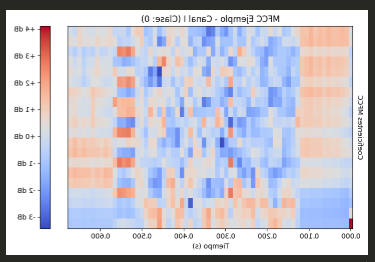
\includegraphics[width=8cm,height=8cm]{input.png}};

\pic[shift={ (0,0,0) }] at (1,0,0) 
    {Box={
        name=flat,
        caption=Flatten,
        fill=\UnpoolColor,
        opacity=0.5,
        height=32,
        width=3,
        depth=32
        }
    };

\pic[shift={(0,0,0)}] at (4,0,0) 
    {Box={
        name=linear,
        caption=Linear,
        xlabel={{1280, }},
        zlabel=,
        fill=\ConvColor,
        height=32,
        width=3,
        depth=32
        }
    };

\draw [connection]  (flat-east)    -- node {\midarrow} (linear-west);

\pic[shift={ (2,0,0) }] at (linear-east) 
    {RightBandedBox={
        name=fc1,
        caption=FC1,
        xlabel={{ "~~~256 256" , }},
        zlabel=,
        fill=\ConvColor,
        bandfill=\ConvReluColor,
        height=22,
        width={ 3 , 3 },
        depth=22
        }
    };

\draw [connection]  (linear-east)    -- node {\midarrow} (fc1-west);

\pic[shift={ (0,0,0) }] at (fc1-east) 
    {Box={
        name=pool2,
        caption= ,
        fill=\PoolColor,
        opacity=0.5,
        height=12,
        width=1,
        depth=12
        }
    };

\pic[shift={ (1,0,0) }] at (pool2-east) 
    {RightBandedBox={
        name=fc2,
        caption=FC2,
        xlabel={{ 64, 64 }},
        zlabel=,
        fill=\ConvColor,
        bandfill=\ConvReluColor,
        height=10,
        width={ 3 , 3 },
        depth=10
        }
    };

\draw [connection]  (pool2-east)    -- node {\midarrow} (fc2-west);

\pic[shift={ (0,0,0) }] at (fc2-east) 
    {Box={
        name=pool3,
        caption= ,
        fill=\PoolColor,
        opacity=0.5,
        height=6,
        width=1,
        depth=6
        }
    };

\pic[shift={(2,0,0)}] at (pool3-east) 
    {Box={
        name=soft1,
        caption= \\~\\Spkr.\\ Recognition,
        xlabel={{10,"dummy"}},
        zlabel=,
        fill=\SoftmaxColor,
        opacity=0.8,
        height=3,
        width=1.5,
        depth=25
        }
    };

\draw [connection]  (pool3-east)    -- node {\midarrow} (soft1-west);

\end{tikzpicture}
\end{document}
